% ESPARGOS T-Dongle-C5 Test Transmitter  -  User Manual
% Build:  xelatex manual.tex   (three times for cross-references)
%         make                  (via Makefile)
%
% This manual documents the LILYGO T-Dongle-C5 based WiFi test transmitter for
% ESPARGOS channel measurement experiments. It deliberately mirrors the visual
% style of the other ESPARGOS manuals (Quick Start Manual, Aperture Kit
% supplement).

\documentclass[a5paper, 10pt, twoside]{article}

%%──────────────────────────────────────────────────────────────────────────
%%  PACKAGES
%%──────────────────────────────────────────────────────────────────────────
\usepackage{fontspec}
\usepackage[a5paper, twoside,
  top=20mm, bottom=13mm, inner=13mm, outer=15mm,
  headheight=13pt, headsep=5mm, footskip=6mm
]{geometry}
\usepackage{xcolor}
\usepackage{graphicx}
\usepackage{float}
\usepackage{caption}
\usepackage{subcaption}
\usepackage{tikz}
\usetikzlibrary{calc, positioning, shapes, arrows, arrows.meta, backgrounds}
\usepackage{adjustbox}
\usepackage[most]{tcolorbox}
\usepackage{booktabs}
\usepackage{enumitem}
\usepackage{microtype}
\usepackage{tabularx}
\usepackage{array}
\usepackage{xfrac}
\usepackage{fancyhdr}
\usepackage{titlesec}
\usepackage[hidelinks]{hyperref}
\usepackage{parskip}
\usepackage{listings}
\usepackage{needspace}
\usepackage{eso-pic}

%%──────────────────────────────────────────────────────────────────────────
%%  FONTS
%%──────────────────────────────────────────────────────────────────────────
\setmainfont{Carlito}
\setsansfont{Carlito}
\setmonofont[Scale=0.86]{Source Code Pro}

%%──────────────────────────────────────────────────────────────────────────
%%  COLORS
%%──────────────────────────────────────────────────────────────────────────
\definecolor{espgreen}{HTML}{37c964}
\definecolor{espgreendark}{HTML}{227b3d}
\definecolor{espdark}{HTML}{293135}
\definecolor{espgreenlight}{HTML}{d7f4e0}
\definecolor{espgreenbg}{HTML}{edfbf2}
\definecolor{espwarningbg}{HTML}{fff8e1}
\definecolor{espwarning}{HTML}{c87000}
\definecolor{espred}{HTML}{dc3545}
\definecolor{esplightgray}{HTML}{f4f4f4}
\definecolor{espcodefg}{HTML}{1a2a1a}
\definecolor{esptextgray}{HTML}{4a5550}
\definecolor{esprulegray}{HTML}{d0d8d4}
%% Transmitter index accent colors (same palette as the firmware / pyespargos)
\definecolor{txblue}{HTML}{1f77b4}
\definecolor{txorange}{HTML}{ff7f0e}
\definecolor{txgreen}{HTML}{2ca02c}
\definecolor{txred}{HTML}{d62728}
\definecolor{txpurple}{HTML}{9467bd}

%%──────────────────────────────────────────────────────────────────────────
%%  FIGURE CAPTIONS  (scientific-paper style: numbered + referenced)
%%──────────────────────────────────────────────────────────────────────────
\captionsetup{
  font         = {footnotesize, color=esptextgray},
  labelfont    = {bf, color=espgreendark},
  textfont     = {it},
  labelsep     = period,
  justification= centering,
  skip         = 4pt,
}

%%──────────────────────────────────────────────────────────────────────────
%%  HYPERREF
%%──────────────────────────────────────────────────────────────────────────
\hypersetup{
  colorlinks = true,
  linkcolor  = espdark,
  urlcolor   = espgreendark,
  pdfauthor  = {TTI GmbH / TGU ESPARGOS},
  pdftitle   = {ESPARGOS T-Dongle-C5 Test Transmitter - User Manual},
}

%%──────────────────────────────────────────────────────────────────────────
%%  COLORED BOXES
%%──────────────────────────────────────────────────────────────────────────
\tcbuselibrary{skins, breakable}

%% Note box  ─  green left stripe, subtle green tint
\newtcolorbox{notebox}[1][Note]{%
  enhanced, breakable,
  colback  = espgreenbg,
  colframe = espgreen,
  leftrule = 3.5pt, rightrule = 0.5pt, toprule = 0.5pt, bottomrule = 0.5pt,
  arc = 2pt, outer arc = 2pt,
  before skip = 6pt, after skip = 6pt,
  left = 6pt, right = 5pt, top = 4pt, bottom = 4pt,
  fontupper = \small,
  before upper = {%
    \leavevmode\textcolor{espgreendark}{\bfseries\footnotesize #1\enspace}%
  },
}

%% Warning box  ─  amber left stripe, warm tint
\newtcolorbox{warnbox}[1][Warning]{%
  enhanced, breakable,
  colback  = espwarningbg,
  colframe = espwarning,
  leftrule = 3.5pt, rightrule = 0.5pt, toprule = 0.5pt, bottomrule = 0.5pt,
  arc = 2pt, outer arc = 2pt,
  before skip = 6pt, after skip = 6pt,
  left = 6pt, right = 5pt, top = 4pt, bottom = 4pt,
  fontupper = \small,
  before upper = {%
    \leavevmode\textcolor{espwarning}{\bfseries\footnotesize #1\enspace}%
  },
}

%%──────────────────────────────────────────────────────────────────────────
%%  LISTINGS
%%──────────────────────────────────────────────────────────────────────────
\lstdefinestyle{espstyle}{
  basicstyle    = \ttfamily\scriptsize\color{espcodefg},
  backgroundcolor = \color{esplightgray},
  rulecolor     = \color{esprulegray},
  frame         = single, framesep = 3pt, framerule = 0.6pt,
  breaklines    = true, breakatwhitespace = true,
  showstringspaces = false,
  keywordstyle  = \color{espgreendark}\bfseries,
  stringstyle   = \color{espdark!70},
  commentstyle  = \color{esptextgray}\itshape,
  aboveskip = 4pt, belowskip = 4pt,
  xleftmargin = 2pt, xrightmargin = 2pt,
}
\lstset{style=espstyle}

%%──────────────────────────────────────────────────────────────────────────
%%  SECTION HEADINGS
%%──────────────────────────────────────────────────────────────────────────
%% Thick green vertical accent bar to the left of the heading text.
\titleformat{\section}[block]
  {\large\bfseries\color{espdark}}
  {}{0pt}
  {{\color{espgreen}\rule[-2.5pt]{3.5pt}{15pt}}\hspace{7pt}}
\titlespacing*{\section}{0pt}{13pt}{6pt}

\titleformat{\subsection}[block]
  {\normalsize\bfseries\color{espdark}}
  {}{0pt}{}
\titlespacing*{\subsection}{0pt}{7pt}{2pt}

\titleformat{\subsubsection}[block]
  {\small\bfseries\color{espgreendark}}
  {}{0pt}{}
\titlespacing*{\subsubsection}{0pt}{6pt}{1pt}

%%──────────────────────────────────────────────────────────────────────────
%%  HEADERS / FOOTERS
%%──────────────────────────────────────────────────────────────────────────
\pagestyle{fancy}
\fancyhf{}
\fancyhead[LE,RO]{\footnotesize\color{esptextgray}\thepage}
\fancyhead[RE,LO]{\footnotesize\color{esptextgray}%
  \textcolor{espgreen}{\bfseries ESPARGOS Test Transmitter}\enspace User Manual}
\makeatletter
\renewcommand{\headrule}{%
  {\color{espgreen}\hrule \@height 1.5pt \@width \headwidth}%
  \vspace{1.5pt}%
}
\renewcommand{\headrulewidth}{1.5pt}
\makeatother

%%──────────────────────────────────────────────────────────────────────────
%%  UTILITY COMMANDS
%%──────────────────────────────────────────────────────────────────────────
\newcommand{\espname}{\textcolor{espgreen}{\textbf{ESPARGOS}}}
\newcommand{\espdongle}{\textcolor{espgreen}{\textbf{T-Dongle-C5 Test Transmitter}}}
\newcommand{\manualrev}{1.0}
\newcommand{\manualdate}{July 2026}
\newcommand{\manualrevision}{Rev~\manualrev, \manualdate}
\setlength{\parskip}{3pt plus 1pt}
\setlength{\parindent}{0pt}

%%──────────────────────────────────────────────────────────────────────────
%%  COVER BACKGROUND HELPER
%%──────────────────────────────────────────────────────────────────────────
\newcommand{\coverpagesetup}{%
  \thispagestyle{empty}%
  \newgeometry{margin=0pt}%
}

%%──────────────────────────────────────────────────────────────────────────
\begin{document}
\raggedbottom

%%══════════════════════════════════════════════════════════════════════════
%%  PAGE 1 - FRONT COVER
%%══════════════════════════════════════════════════════════════════════════
\coverpagesetup

\begin{tikzpicture}[remember picture, overlay]
  %% Full light background
  \fill[white] (current page.south west) rectangle (current page.north east);

  %% Top green accent stripe
  \fill[espgreen] ([yshift=-25mm]current page.north west)
    rectangle ([yshift=-27mm]current page.north east);

  %% Logo
  \node[anchor=west] at ([xshift=10mm, yshift=-16mm]current page.north west)
    {
\includegraphics[height=14mm]{img/espargos-logo.pdf}};

  %% Green glow behind/underneath the product image
  \shade[inner color=espgreen!40, outer color=white]
    ([xshift=0mm, yshift=-102mm]current page.north)
    ellipse (60mm and 32mm);

  %% Product image - centered on page
  \node[anchor=center]
    at ([xshift=0mm, yshift=-100mm]current page.north)
    {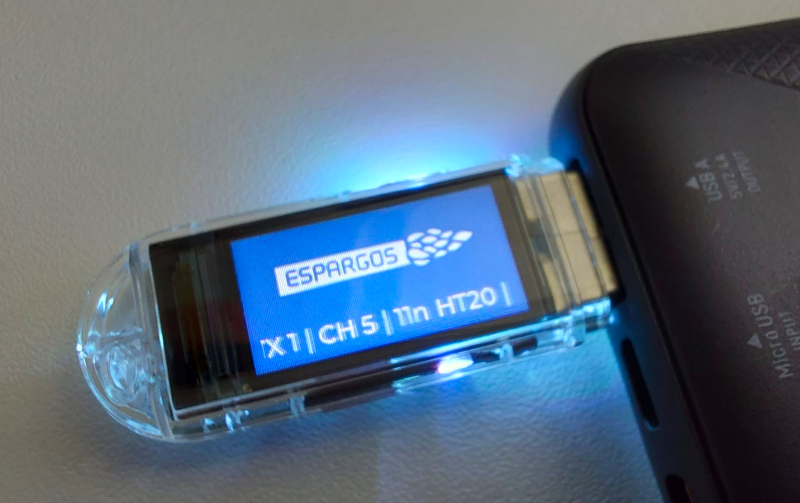
\includegraphics[width=112mm]{img/dongle-in-powerbank.png}};

  %% Model name
  \node[anchor=north, text=espdark,
        font=\fontsize{22}{26}\bfseries\selectfont]
    at ([yshift=-152mm]current page.north)
    {\textcolor{black}{\textbf{Test Transmitter}}};

  %% Bottom green accent band
  \fill[espgreen] ([yshift=24mm]current page.south west)
    rectangle ([yshift=26mm]current page.south east);

  %% Tagline
  \node[anchor=south, text=espdark,
        font=\fontsize{12}{14}\bfseries\selectfont]
    at ([yshift=13mm]current page.south)
    {A Portable WiFi Test Signal Source};

  %% Label
  \node[anchor=south, text=esptextgray,
        font=\fontsize{7.5}{9}\selectfont]
    at ([yshift=6mm]current page.south)
    {User Manual \enspace·\enspace \manualrevision};
\end{tikzpicture}

\clearpage
\restoregeometry

%%══════════════════════════════════════════════════════════════════════════
%%  PAGE 2 - DOCUMENT INFO
%%══════════════════════════════════════════════════════════════════════════
\thispagestyle{empty}
\vspace*{\fill}
\begin{center}
  {\large\bfseries\color{espdark} ESPARGOS T-Dongle-C5 Test Transmitter}\\[4pt]
  {\normalsize\color{esptextgray} User Manual}\\[18pt]
  \begin{tabular}{@{}rl@{}}
    \textbf{Revision:} & \manualrev \\[3pt]
    \textbf{Date:}     & \manualdate \\
  \end{tabular}\\[24pt]
  \textcolor{esptextgray}{\small TTI GmbH / TGU ESPARGOS}
\end{center}

\vspace{22pt}
\begin{center}
\begin{tcolorbox}[enhanced, breakable=false,
  colback = espgreenbg, colframe = espgreen,
  boxrule = 0.9pt, arc = 4pt, outer arc = 4pt,
  left = 14pt, right = 14pt, top = 9pt, bottom = 9pt,
  width = 0.78\linewidth, halign = center]
  {\footnotesize\bfseries\color{esptextgray}Firmware \& source code}\\[5pt]
  {\normalsize\bfseries\begingroup\hypersetup{urlcolor=espdark}%
   \href{https://github.com/ESPARGOS/t-dongle-c5-transmitter}%
        {\texttt{github.com/ESPARGOS/}\\\texttt{t-dongle-c5-transmitter}}\endgroup}\\[8pt]
  {\footnotesize\bfseries\color{esptextgray}Questions?}\\[4pt]
  {\normalsize\bfseries\begingroup\hypersetup{urlcolor=espdark}%
   \href{mailto:info@espargos.net}{\texttt{info@espargos.net}}\endgroup}
\end{tcolorbox}
\end{center}
\vspace*{\fill}

\clearpage

%%══════════════════════════════════════════════════════════════════════════
%%  OVERVIEW
%%══════════════════════════════════════════════════════════════════════════
\section{Overview}
\label{sec:overview}

The \espdongle{} is a WiFi test transmitter for experiments with \espname{}
antenna arrays. It runs on a LILYGO T-Dongle-C5 (ESP32-C5) and continuously
transmits \textbf{broadcast 802.11 data frames} at a configurable interval.
These frames serve as known test signals: every frame that an \espname{} array
receives yields one channel measurement (CSI). The transmitter never joins a
WiFi network and never acts as an access point; it simply keeps sending frames
on a fixed 2.4\,GHz channel.

The dongle is powered over USB: plugged into a \textbf{power bank}
(Figure~\ref{fig:dongle-photo}), it becomes a fully portable test transmitter
that you can carry around the room.

\begin{figure}[H]
  \centering
  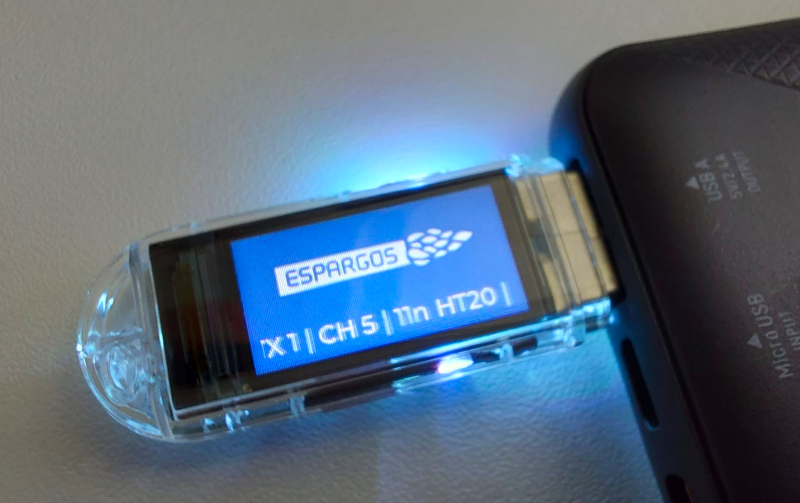
\includegraphics[width=0.54\linewidth]{img/dongle-in-powerbank.png}
  \caption{The \espdongle{} plugged into a power bank, showing the active
  configuration on its display.}
  \label{fig:dongle-photo}
\end{figure}

All transmission parameters, i.e., channel, modulation, rate, packet interval
and transmit power, can be changed \textbf{directly on the device} using its
single button and built-in display (Section~\ref{sec:controls}); no serial
console or computer is needed. Settings are stored in flash and survive
reboots and power loss.

\subsection{Transmitter Index}
When you use several test transmitters at once, the \textbf{TX index}
(1--5) tells them apart. The index is embedded in the last byte of the
transmitter's MAC address (source address and BSSID), so the receiving side
can distinguish the transmitters by MAC address. Each index also has a fixed
accent color, shown on the dongle's LED and display background:

\begin{center}
\begin{tabular}{@{}cccccc@{}}
\toprule
\textbf{TX index} & 1 & 2 & 3 & 4 & 5 \\
\midrule
\textbf{Color} &
\textcolor{txblue}{\rule{8mm}{3mm}} &
\textcolor{txorange}{\rule{8mm}{3mm}} &
\textcolor{txgreen}{\rule{8mm}{3mm}} &
\textcolor{txred}{\rule{8mm}{3mm}} &
\textcolor{txpurple}{\rule{8mm}{3mm}} \\
\bottomrule
\end{tabular}
\end{center}

%%══════════════════════════════════════════════════════════════════════════
%%  CONTROLS
%%══════════════════════════════════════════════════════════════════════════
\clearpage
\section{On-Device Controls}
\label{sec:controls}

After a short splash screen, the dongle shows the \textbf{home screen}: the
ESPARGOS logo on the accent-colored background and a scrolling status line
with the complete active configuration, for example:

\begin{center}
\texttt{\small TX 1 | CH 5 | 11n HT20 | MCS0 | INT 20ms | PWR 20.00dBm}
\end{center}

Everything is controlled with the \textbf{single button} on the dongle. A
\emph{short press} always means ``next'', a \emph{long press}
($\geq$\,0.6\,s) always means ``enter / apply'':

\begin{figure}[H]
\centering
\begin{adjustbox}{max width=\linewidth, keepaspectratio}
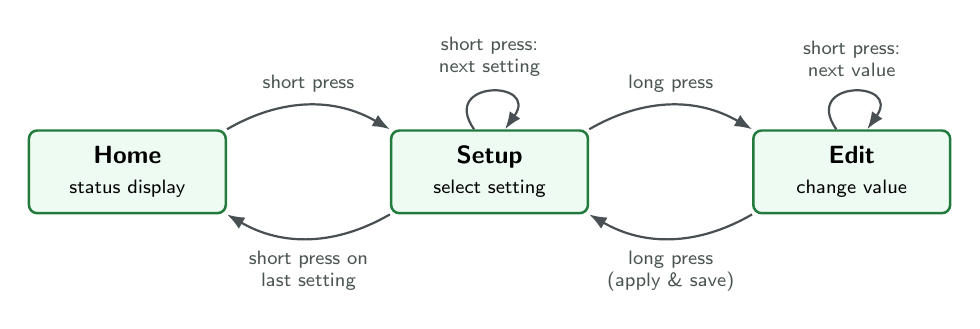
\begin{tikzpicture}[
  font=\sffamily\small,
  state/.style={draw=espgreendark, fill=espgreenbg, rounded corners=3pt,
                line width=0.9pt, minimum width=2.5cm, minimum height=1.05cm,
                align=center},
  press/.style={-{Latex[length=2.2mm]}, thick, espdark!85},
  presslbl/.style={font=\scriptsize\sffamily, text=esptextgray, align=center},
]
\node[state] (home)  at (0,0)   {\textbf{Home}\\{\scriptsize status display}};
\node[state] (setup) at (4.6,0) {\textbf{Setup}\\{\scriptsize select setting}};
\node[state] (edit)  at (9.2,0) {\textbf{Edit}\\{\scriptsize change value}};

%% Transitions between states: enter/leave the menu, enter/leave edit mode
\draw[press] (home.north east) to[bend left=30]
  node[presslbl, above=1pt] {short press} (setup.north west);
\draw[press] (setup.south west) to[bend left=30]
  node[presslbl, below=1pt] {short press on\\last setting} (home.south east);

\draw[press] (setup.north east) to[bend left=30]
  node[presslbl, above=1pt] {long press} (edit.north west);
\draw[press] (edit.south west) to[bend left=30]
  node[presslbl, below=1pt] {long press\\(apply \& save)} (setup.south east);

%% Self-loops on top of Setup and Edit: short press cycles in place
\draw[press] (setup.110) to[out=125, in=55, looseness=5]
  node[presslbl, above=2pt] {short press:\\next setting} (setup.70);
\draw[press] (edit.110) to[out=125, in=55, looseness=5]
  node[presslbl, above=2pt] {short press:\\next value} (edit.70);
\end{tikzpicture}
\end{adjustbox}
\caption{The on-device menu. A short press cycles (through settings in
\emph{Setup}, through values in \emph{Edit}), a long press goes deeper
(\emph{Setup} $\rightarrow$ \emph{Edit}) or applies and saves the edited
value (\emph{Edit} $\rightarrow$ \emph{Setup}).}
\label{fig:menu-flow}
\end{figure}

In detail:

\begin{itemize}[leftmargin=1.5em, itemsep=2pt, topsep=2pt]
  \item \textbf{Home screen, short press:} opens the setup menu.
  \item \textbf{Setup menu (header \texttt{SETUP k/n}):} a short press moves
        to the next setting; after the last setting it returns to the home
        screen. A long press starts editing the displayed setting.
  \item \textbf{Edit mode (header \texttt{EDIT k/n}):} a short press cycles
        to the next value of the setting; a long press applies the new value,
        stores it permanently and returns to the setup menu.
  \item While the button is held down, the header previews what the long
        press will do (\texttt{EDIT} or \texttt{APPLY}), so you can release
        with confidence.
\end{itemize}

\begin{notebox}
The transmitter \textbf{keeps transmitting} with its active configuration
while you navigate the menu. An edited value only takes effect at the moment
you apply it with a long press.
\end{notebox}

%%══════════════════════════════════════════════════════════════════════════
%%  SETTINGS
%%══════════════════════════════════════════════════════════════════════════
\clearpage
\section{Settings Reference}
\label{sec:settings}

The setup menu offers the following settings, in this order. The
\emph{Secondary} entry only appears when the modulation is 802.11n HT40.

\vspace{2pt}
{\footnotesize
\setlength{\tabcolsep}{5pt}
\renewcommand{\arraystretch}{1.3}
\begin{tabularx}{\linewidth}{@{}>{\bfseries\raggedright\arraybackslash}p{2.0cm}
  >{\raggedright\arraybackslash}p{3.2cm}
  >{\raggedright\arraybackslash}X@{}}
\toprule
\textbf{Setting} & \textbf{Values} & \textbf{Notes} \\
\midrule
Channel     & 1--13 &
  2.4\,GHz band. With HT40: 1--9 (secondary above) or 5--13 (secondary
  below). \\
TX Index    & 1--5 &
  Sets the last MAC address byte and the accent color
  (Section~\ref{sec:overview}). \\
Modulation  & 802.11b, 802.11g, 11n HT20, 11n HT40, 11ax HE20 &
  PPDU format of the transmitted frames. HT40 uses a 40\,MHz channel, all
  others 20\,MHz. \\
Rate        & depends on modulation &
  802.11b: 1\,/\,2\,/\,5.5\,/\,11\,Mbps; 802.11g: 6--54\,Mbps;
  HT20\,/\,HT40: MCS\,0--7; HE20: MCS\,0--9. \\
Secondary   & Above, Below &
  Position of the secondary 20\,MHz channel (HT40 only). \\
Interval    & 1\,ms--1000\,ms &
  Time between frames, from a preset list (1, 2, 5, 7, 10, 11, 13, 15, 16,
  20, 25, 50, 100, 200, 500, 1000\,ms). \\
TX Power    & 2--21\,dBm &
  Maximum transmit power, in steps of 2\,dBm (plus a 21\,dBm top setting). \\
\bottomrule
\end{tabularx}
}

\begin{notebox}
Applied settings are stored in non-volatile flash memory (NVS) and are
restored on the next boot. To reset the transmitter to its compiled-in
defaults, erase the flash (\texttt{idf.py erase-flash}) and flash the
firmware again.
\end{notebox}

\begin{warnbox}[Match the ESPARGOS Channel Configuration]
For CSI measurements the transmitter's channel settings must match the
receiving \espname{} arrays: same primary channel and, when transmitting
HT40, a secondary channel position that overlaps the arrays' configuration.
A channel mismatch is the most common reason for ``no CSI received''.
\end{warnbox}

%%══════════════════════════════════════════════════════════════════════════
%%  FIRMWARE
%%══════════════════════════════════════════════════════════════════════════
\clearpage
\section{Firmware}
\label{sec:firmware}

The firmware is open source and available at
\begin{center}
\href{https://github.com/ESPARGOS/t-dongle-c5-transmitter}%
     {\texttt{https://github.com/ESPARGOS/t-dongle-c5-transmitter}}
\end{center}
It is built with \textbf{ESP-IDF} for the ESP32-C5:

\begin{lstlisting}[language=bash]
idf.py set-target esp32c5
idf.py build
idf.py -p /dev/ttyACM0 flash monitor
\end{lstlisting}

Adjust the serial port to your machine. To enter the ESP32-C5 BOOT mode for
flashing, \textbf{hold the button while plugging the dongle in}.

\subsection{Compile-Time Defaults (menuconfig)}
The factory defaults of all transmitter settings can be changed before
compiling with

\begin{lstlisting}[language=bash]
idf.py menuconfig
\end{lstlisting}

under the menu item \textbf{CSI transmitter}. It contains the same settings
as the on-device menu (default modulation, rate\,/\,MCS, channel, secondary
channel, TX index, interval and maximum TX power), with two differences:
the interval accepts any value from 1\,ms to 60\,s (not just the preset
list), and the TX power is given in units of 0.25\,dBm (8--84, default
80\,=\,20\,dBm).

\begin{notebox}
Settings changed on the running device are stored in NVS and
\textbf{override} the menuconfig defaults. The menuconfig values only apply
when no stored configuration exists, i.e., after the flash has been erased.
\end{notebox}

\subsection{Serial Monitor}
The dongle logs its active configuration and per-second packet counters
(transmitted frames, transmit failures, current channel) on the USB serial
console, e.g.\ via \texttt{idf.py monitor}. This is useful to verify that
frames are actually being sent, but it is not required for normal operation.

%%══════════════════════════════════════════════════════════════════════════
%%  NOTES PAGE  (filler so the total page count stays divisible by 4 for
%%  brochure printing; also handy for the reader)
%%══════════════════════════════════════════════════════════════════════════
\clearpage
\section*{Notes}
\vspace{4mm}
\foreach \n in {1,...,11}{%
  \textcolor{esprulegray}{\rule{\linewidth}{0.5pt}}\par\vspace{10.5mm}%
}

%%══════════════════════════════════════════════════════════════════════════
%%  BACK COVER
%%══════════════════════════════════════════════════════════════════════════
\clearpage
\coverpagesetup

\begin{tikzpicture}[remember picture, overlay]
  \fill[white] (current page.south west) rectangle (current page.north east);

  %% Top green accent stripe (mirrors the front cover)
  \fill[espgreen] ([yshift=-25mm]current page.north west)
    rectangle ([yshift=-27mm]current page.north east);

  %% Logo, centered
  \node[anchor=center] at ([yshift=14mm]current page.center)
    {
\includegraphics[height=13mm]{img/espargos-logo.pdf}};

  %% Contact block
  \node[anchor=north, text=esptextgray, align=center,
        font=\small]
    at ([yshift=-2mm]current page.center)
    {Questions?\\[2pt]
     \href{mailto:info@espargos.net}{\texttt{info@espargos.net}}\\[2pt]
     \href{https://espargos.net}{\texttt{https://espargos.net}}};

  %% Bottom green accent band
  \fill[espgreen] ([yshift=24mm]current page.south west)
    rectangle ([yshift=26mm]current page.south east);

  %% Label
  \node[anchor=south, text=esptextgray,
        font=\fontsize{7.5}{9}\selectfont]
    at ([yshift=6mm]current page.south)
    {ESPARGOS T-Dongle-C5 Test Transmitter \enspace·\enspace
     User Manual \enspace·\enspace \manualrevision};
\end{tikzpicture}

\end{document}
